% Provenance (never printed): see sources/outline_sources.md (Year 2: Hadean, Archean and
% Proterozoic; early crust and greenstone belts; the oxygenation of the atmosphere; snowball
% Earth). Eons and eras from the ICS chart; greenstone belts, TTG and cratons after Cawood and
% others (2018) and Smithies and others (2019); komatiite liquidus after Sossi and O'Neill (2016),
% Pierru and others (2022) and Asimow (2022); the Archean air and the GOE after Catling and Zahnle
% (2020) and Luo and others (2016); the boring billion after Lyons and others (2021); snowball
% Earth after Hoffman and others (2017). The energy-balance model, the komatiite line and the CO2
% build-up from figdata/bachelor-2/precambrian.py; exercise and problem values in the Book 4
% scratch calculator calc/ch18.py.
\chapter{La Tierra precámbrica}\label{ch:b2:precambrian-earth}

Los primeros fósiles con concha aparecen en rocas de unos 540 millones de años. Todo lo anterior, desde
el nacimiento de la Tierra hace \qty{4567}{Ma}, es el Precámbrico: siete octavos de la historia del
planeta. En ese tiempo la Tierra construyó los núcleos de sus continentes, llenó su aire de oxígeno
y al menos dos veces se heló de los polos al ecuador, con casquetes de hielo que llegaban al mar
en los trópicos. Este capítulo lee esos cuatro mil millones de años en las rocas que han sobrevivido de ellos,
y pone cifras a tres de sus enigmas: por qué las lavas más antiguas eran tan calientes, cómo puede deshelarse un
planeta congelado y cómo se mantuvo caliente la Tierra joven bajo un Sol débil.
% ledger: ics:base.Hadean, ics:base.Phanerozoic, hoffman17:cryochrons

\begin{recall}
\textbf{De los volúmenes escolares}: la edad de la Tierra; los eones de la escala de tiempo geológico;
la ley de luminosidad del Sol joven y la \omterm{def:b2:precambrian-earth:faint-sun}{paradoja del Sol joven débil}; la atmósfera primitiva;
los estromatolitos, las formaciones de hierro bandeado, el \omterm{def:b2:precambrian-earth:goe}{Gran Evento de Oxidación} y las capas rojas; los cratones;
el calor radiogénico en el pasado. \textbf{Del volumen de primer año}: el circón y sus edades U--Pb, la
temperatura de cierre; la producción de calor radiogénico de los cuatro isótopos; la radiación de onda larga
saliente y la insolación media global $S_0/4$; las unidades cronoestratigráficas.
\textbf{De capítulos anteriores}: la \omterm{def:b2:mantle-melting:tp}{temperatura potencial del manto} y la adiabática
(\cref{ch:b2:mantle-melting}); el liquidus y la \omterm{def:b2:magmatic-differentiation:crystallisation}{cristalización fraccionada} del olivino
(\cref{ch:b2:magmatic-differentiation}); los tipos de granito (\cref{ch:b2:crustal-melting});
los \omterm{def:b2:wilson-cycle:supercontinent}{supercontinentes} (\cref{ch:b2:wilson-cycle}). La oxidación y la reducción corresponden a los libros de
química, y los primeros eucariotas y la fotosíntesis, a los de biología.
\end{recall}

\section{Tres eones antes de los fósiles}\label{sec:b2:precambrian-earth:eons}

\begin{definition}[Hádico, Arcaico, Proterozoico]\label{def:b2:precambrian-earth:eons}
El tiempo anterior al Fanerozoico se divide en tres eones. El \emph{Hádico}\index{Hadico@Hádico}
va desde la formación de la Tierra, hace \qty{4567}{Ma}, hasta $4031 \pm \qty{3}{Ma}$; el
\emph{Arcaico}\index{Arcaico}, de $4031$ a \qty{2500}{Ma}; el
\emph{Proterozoico}\index{Proterozoico}, de 2500 a \qty{538.8}{Ma}, la base del Cámbrico.
En conjunto se llaman informalmente Precámbrico.
\end{definition}
% ledger: ics:base.Hadean, ics:base.Archean, ics:base.Proterozoic, ics:base.Phanerozoic

El \omterm{def:b2:precambrian-earth:eons}{Arcaico} se divide en cuatro eras, el Eoarcaico (4031 a \qty{3600}{Ma}), el Paleoarcaico (3600
a 3200), el Mesoarcaico (3200 a 2800) y el Neoarcaico (2800 a 2500); el \omterm{def:b2:precambrian-earth:eons}{Proterozoico}, en tres,
el Paleoproterozoico (2500 a \qty{1600}{Ma}), el Mesoproterozoico (1600 a 1000) y el
Neoproterozoico (1000 a 538.8). Dos periodos del Neoproterozoico importan más adelante, el Criogénico, de 720 a
\qty{635}{Ma}, y el Ediacárico, de 635 a \qty{538.8}{Ma}.
% ledger: ics4:archean-eras, ics4:proterozoic-eras

\begin{omfigure}
\centering
% ledger: ics:base.Hadean, ics:base.Archean, ics:base.Proterozoic, ics:base.Phanerozoic, ics4:archean-eras, ics4:proterozoic-eras, wilde01:4404, bowring99:acasta, cz20:impacts, allwood06:spc, cawood18:transition, gumsley17:goe, luo16:goe, hoffman17:earlier, earle:bif, lyons21:boring, hoffman17:ages, asimow22:komatiite
\begin{tikzpicture}[x=-3.4cm, y=1cm, font=\scriptsize]
% eons
\fill[icsHadean] (4.567,0) rectangle (4.031,0.5);
\fill[icsArchean] (4.031,0) rectangle (2.5,0.5);
\fill[icsProterozoic] (2.5,0) rectangle (0.5388,0.5);
\fill[icsPhanerozoic] (0.5388,0) rectangle (0,0.5);
\node[text=white] at (4.299,0.25) {Hádico};
\node[text=white] at (3.27,0.25) {Arcaico};
\node[text=white] at (1.52,0.25) {Proterozoico};
\node at (0.27,0.25) {Fan.};
% eras
\foreach \a/\b/\c in {4.031/3.6/35, 3.6/3.2/55, 3.2/2.8/35, 2.8/2.5/55}
  \fill[icsArchean!\c] (\a,-0.45) rectangle (\b,0);
\foreach \a/\b/\c in {2.5/1.6/35, 1.6/1.0/55, 1.0/0.5388/35}
  \fill[icsProterozoic!\c] (\a,-0.45) rectangle (\b,0);
\foreach \x/\l in {3.8155/Eo, 3.4/Paleo, 3.0/Meso, 2.65/Neo, 2.05/Paleo, 1.3/Meso, 0.769/Neo}
  \node at (\x,-0.225) {\l};
% axis
\draw (4.6,-0.6) -- (0,-0.6);
\foreach \t in {0,0.5,...,4.5} {
  \draw (\t,-0.6) -- (\t,-0.7);
  \node[anchor=north] at (\t,-0.7) {\pgfmathprintnumber[fixed, precision=1]{\t}};
}
\node[anchor=north, font=\small] at (2.3,-1.05) {tiempo antes del presente (miles de millones de años)};
% row A
\fill[omDef] (4.404,0.85) circle (2pt);
\node[anchor=west, text=omDef] at (4.404,0.85) {circón más antiguo};
\fill[omMeth] (3.43,0.85) circle (2pt);
\node[anchor=west, text=omMeth] at (3.43,0.85) {primeros estromatolitos};
\draw[red!60!black, line width=3pt] (2.4,0.85) -- (1.8,0.85);
\node[anchor=west, text=red!60!black] at (1.8,0.85) {formaciones de hierro bandeado};
% row B
\fill[omDef] (4.03,1.5) circle (2pt);
\node[anchor=west, text=omDef] at (4.03,1.5) {rocas más antiguas};
\draw[black!70, line width=3pt] (3.2,1.5) -- (2.5,1.5);
\node[anchor=south, text=black!80] at (2.85,1.6) {cambio de estilo tectónico};
\draw[omProp, line width=3pt] (1.8,1.5) -- (0.8,1.5);
\node[anchor=south, text=omProp] at (1.3,1.6) {«mil millones aburridos»};
% row C
\draw[black!60, line width=2pt, densely dashed] (4.2,2.25) -- (3.5,2.25);
\node[anchor=south, text=black!70] at (3.85,2.35) {¿bombardeo intenso tardío? (discutido)};
\draw[omThm, line width=3pt] (2.43,2.25) -- (2.06,2.25);
\node[anchor=west, text=omThm] at (2.06,2.25) {Gran Evento de Oxidación};
% row D
\fill[blue!60!black] (2.4,3.0) circle (2pt);
\node[anchor=east, text=blue!60!black] at (2.4,3.0) {primera Tierra bola de nieve};
\fill[omThm] (0.8,3.0) circle (2pt);
\node[anchor=east, text=omThm] at (0.8,3.0) {segundo aumento del oxígeno};
% row E
\fill[orange!80!black] (1.9,3.7) circle (2pt);
\node[anchor=east, text=orange!80!black] at (1.9,3.7) {últimas komatiitas comunes};
\draw[blue!60!black, line width=3pt] (0.717,3.7) -- (0.635,3.7);
\node[anchor=east, text=blue!60!black] at (0.717,3.7) {bolas de nieve criogénicas};
% row F
\fill[omMeth] (0.57,4.4) circle (2pt);
\node[anchor=east, text=omMeth] at (0.57,4.4) {primeros fósiles grandes (Ediacárico)};
\end{tikzpicture}
\par\smallskip{\small El Precámbrico en una línea. Los eones y, en tonos más claros, sus eras
(Eo-, Paleo-, Meso- y Neoarcaico; Paleo-, Meso- y Neoproterozoico) son los de la
Tabla Cronoestratigráfica Internacional; los acontecimientos se sitúan en las edades citadas en el texto.
Las «últimas \omterm{def:b2:precambrian-earth:greenstone}{komatiitas} comunes» son las no empobrecidas en aluminio; existen tipos más jóvenes y raros.}
\end{omfigure}

\subsection*{El Hádico: minerales sin rocas}

No sobrevive ninguna roca del \omterm{def:b2:precambrian-earth:eons}{Hádico}, solo minerales. El más antiguo es un grano de circón de Jack
Hills, en Australia Occidental, de $4404 \pm \qty{8}{Myr}$, arrancado de una roca más antigua y depositado
en un conglomerado hace unos tres mil millones de años. Su composición, y la de sus
vecinos, fue interpretada por sus descubridores como prueba de que ya existían una corteza de tipo continental y
agua líquida hace \qty{4.4}{Gyr}, unos 160 millones de años después de la formación de la
Tierra. Las rocas datadas más antiguas, los gneises de Acasta, en el noroeste de Canadá, tienen de 4.00 a
\qty{4.03}{Ga}, cerca de la base del \omterm{def:b2:precambrian-earth:eons}{Arcaico}.
% ledger: wilde01:4404, wilde01:zircon, uw14:jack-hills, bowring99:acasta

La Tierra joven fue golpeada por grandes cuerpos, como describió el \cref{ch:b2:planet-formation-meteorites}.
Se estima que el último impacto lo bastante grande para vaporizar
todo el océano ocurrió hace unos \qty{4.3}{Ga}. Se ha propuesto un «bombardeo intenso
tardío» posterior, una ráfaga de impactos entre unos 4.2--4.0 y \qty{3.5}{Ga} deducida de las
edades de las rocas lunares y de los choques en los \omterm{def:b2:planet-formation-meteorites:fall-find}{meteoritos}; muchos discuten incluso que fuera un
acontecimiento distinto, y en cualquier caso probablemente no habría esterilizado la Tierra.
% ledger: cz20:impacts

\section{La corteza arcaica}\label{sec:b2:precambrian-earth:archean}

\subsection*{Cinturones de rocas verdes y komatiitas}

La corteza arcaica que sobrevive está hecha de dos clases de terreno, una junto a otra: grandes cuerpos de
gneis granítico gris, rico en sodio, y cinturones más estrechos de rocas volcánicas y sedimentarias alteradas.

\begin{definition}[Cinturón de rocas verdes; komatiita]\label{def:b2:precambrian-earth:greenstone}
Un \emph{cinturón de rocas verdes}\index{cinturon de rocas verdes@cinturón de rocas verdes} es un cinturón de rocas volcánicas máficas y ultramáficas,
con sedimentos, metamorfizadas en grado bajo (el verde procede de la clorita, la actinolita y la
epidota), situado entre cuerpos de granitoides en terrenos arcaicos y algunos proterozoicos. Una
\emph{komatiita}\index{komatiita} es una lava ultramáfica, mucho más rica en MgO que el basalto,
emitida en estado líquido; su olivino suele crecer en láminas largas y finas, la textura
\emph{spinifex}, al enfriarse deprisa el techo de la colada.
\end{definition}
% ledger: cawood18:dome-keel, so16:liquidus, pierru22:komatiite

\begin{omfigure}
\centering
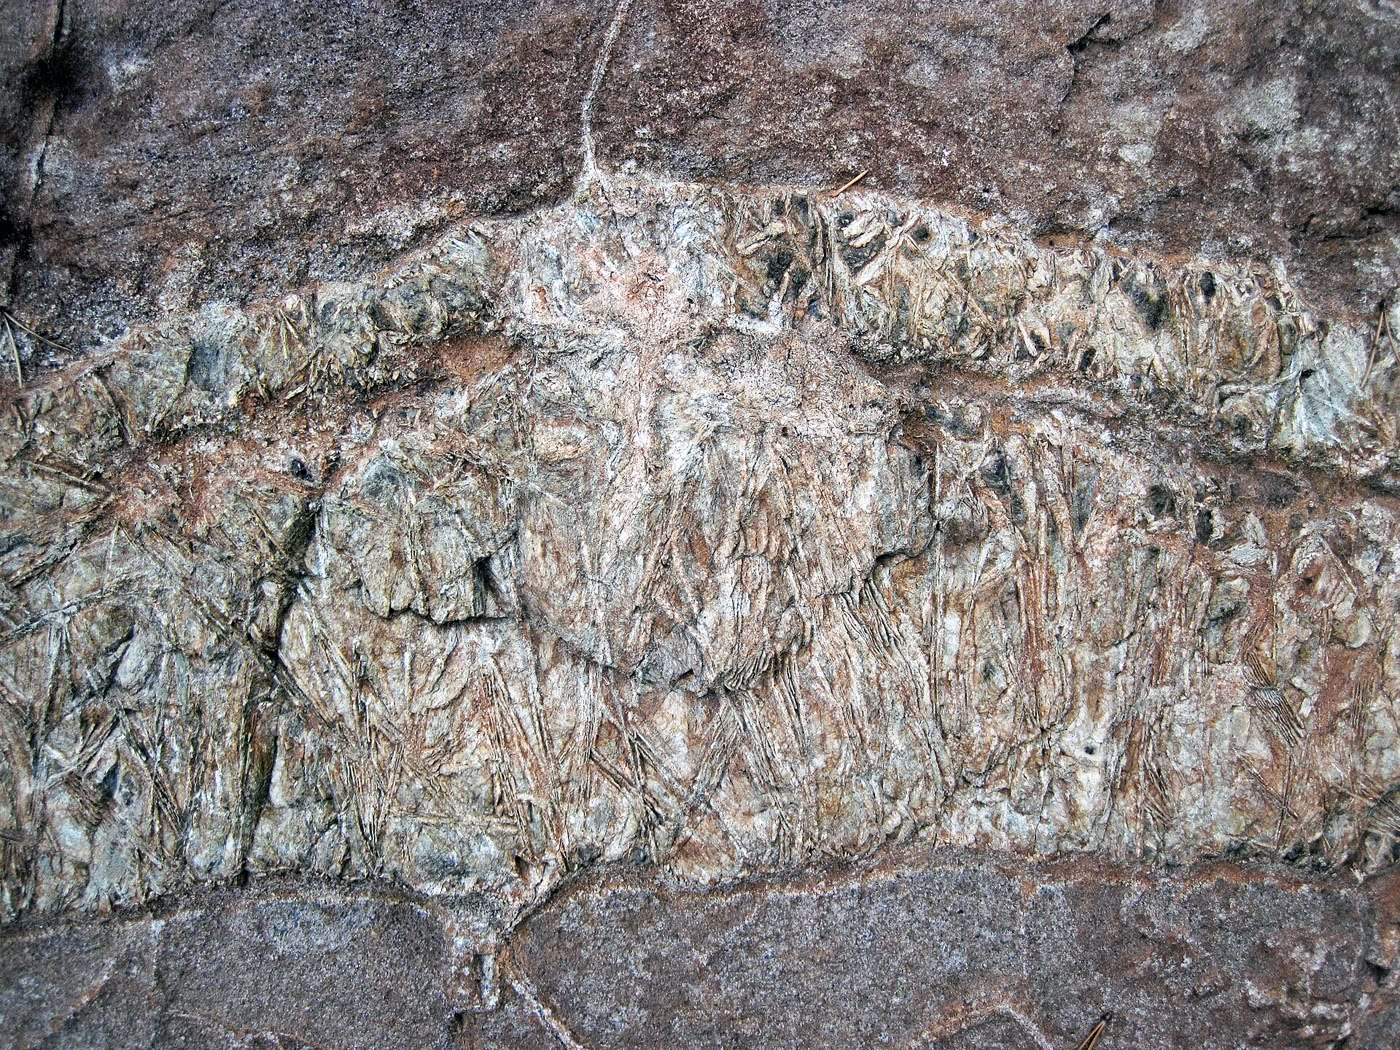
\includegraphics[width=0.66\linewidth]{images/book4/b2-18-spinifex-komatiite.jpg}
\par\smallskip{\small Textura spinifex en una colada de \omterm{def:b2:precambrian-earth:greenstone}{komatiita}, Pyke Hill, Ontario, parte de un
\omterm{def:b2:precambrian-earth:greenstone}{cinturón de rocas verdes} neoarcaico de unos 2710 millones de años: láminas de olivino, hoy alteradas,
crecieron a través del techo de la colada al enfriarse. Fotografía de James St.~John, CC~BY~2.0 (Wikimedia
Commons).}
\end{omfigure}

Las \omterm{def:b2:precambrian-earth:greenstone}{komatiitas} contienen hasta un \qty{34}{\percent} de MgO, frente al 10 a \qty{13}{\percent} de los basaltos
primarios de las dorsales actuales, y están casi limitadas a la Tierra antigua: el tipo empobrecido en aluminio
solo se encuentra en rocas de más de \qty{2.8}{Ga}, el tipo no empobrecido en aluminio hasta unos
\qty{1.9}{Ga}, y solo un raro tipo enriquecido en aluminio llega a ser tan joven como \qty{90}{Myr}. Un fundido
tan rico en magnesio está muy caliente y, como para los basaltos del
\cref{ch:b2:magmatic-differentiation}, el primer mineral que cristaliza de él es el olivino,
cuya proporción en el líquido fija la temperatura.
% ledger: pierru22:komatiite, asimow22:komatiite

\begin{proposition}[El termómetro de las komatiitas]\label{prop:b2:precambrian-earth:liquidus}
Para un fundido en equilibrio con olivino a presión atmosférica, la temperatura de liquidus crece
de forma casi lineal con el contenido en MgO del fundido. Pasando por dos experimentos $(m_1, T_1)$ y
$(m_2, T_2)$,
\[
  T_{\text{liq}}(m) = T_1 + s\,(m - m_1), \qquad s = \frac{T_1 - T_2}{m_1 - m_2} .
\]
Los experimentos de fusión sobre dos \omterm{def:b2:precambrian-earth:greenstone}{komatiitas}, con $\qty{32.2}{\percent}$ de MgO a \qty{1616}{\celsius} y
$\qty{23}{\percent}$ a \qty{1450}{\celsius}, dan $s = \qty{18.0}{\celsius}$ por cada punto porcentual de
MgO.
\end{proposition}
% ledger: so16:liquidus, helz98:glass-thermometer

\begin{proof}
El olivino es una solución sólida de forsterita y fayalita, mucho más rica en magnesio que el fundido
del que crece. Al enfriarse el fundido, el olivino le extrae magnesio, y la temperatura a
la que el fundido está justo saturado en olivino baja con su contenido en MgO. Los experimentos muestran que
en el intervalo de una familia dada de fundidos la caída es casi lineal, de modo que la recta que pasa por
dos experimentos interpola entre ellos; $s = (1616 - 1450)/(32.2 - 23) = 166/9.2 = 18.04$.
\end{proof}

El coeficiente no es exclusivo de las \omterm{def:b2:precambrian-earth:greenstone}{komatiitas}. Los vidrios templados de la lava del Kilauea,
calibrados de la misma manera, varían \qty{3}{\celsius} por cada \qty{0.15}{\percent} de MgO, es
decir, \qty{20}{\celsius} por punto porcentual. Prolongar la recta de las \omterm{def:b2:precambrian-earth:greenstone}{komatiitas} hasta un basalto primario de dorsal
con un \qty{12}{\percent} de MgO da así su liquidus con un margen de unas decenas de grados: $1616 -
18.0\times20.2 \approx \qty{1252}{\celsius}$. Los líquidos komatiíticos más calientes eran, por tanto,
unos \qty{360}{\celsius} más calientes que los fundidos que alimentan las dorsales actuales, y la figura siguiente
muestra la recta.
% ledger: helz98:glass-thermometer, so16:liquidus, pierru22:komatiite
% values: slope 18.043, T_morb12 1251.5, dT_kom_morb 364.5 (precambrian.py)

\begin{omfigure}
\centering
\begin{tikzpicture}
\begin{axis}[omrecord, width=0.72\linewidth, height=6cm, xmin=8, xmax=35, ymin=1150, ymax=1700,
  xlabel={MgO en el fundido (\unit{\percent} en masa)}, ylabel={liquidus a 1 atm (\unit{\celsius})},
  xtick pos=bottom, ytick pos=left, clip=false,
  y tick label style={/pgf/number format/1000 sep={}}]
% computed in figdata/bachelor-2/precambrian.py part kom; ledger: so16:liquidus, pierru22:komatiite
\fill[omProp!15] (axis cs:10,1150) rectangle (axis cs:13,1700);
\addplot[black, line width=1.1pt] table[x=MgO, y=T] {figdata/out/bachelor-2-precambrian-kom.dat};
\addplot[only marks, mark=*, mark size=2.4pt, omThm] coordinates {(32.2,1616) (23,1450)};
\node[anchor=north west, font=\scriptsize, text=omThm] at (axis cs:32.2,1612) {Barberton};
\node[anchor=north west, font=\scriptsize, text=omThm] at (axis cs:23,1446) {Munro};
\node[anchor=south, font=\scriptsize, text=omProp, align=center] at (axis cs:11.5,1560)
  {basaltos primarios\\de dorsal};
\draw[densely dashed] (axis cs:12,1150) -- (axis cs:12,1251.5) -- (axis cs:8,1251.5);
\draw[densely dashed] (axis cs:32.2,1150) -- (axis cs:32.2,1616);
\draw[<->, omDef, thick] (axis cs:27,1251.5) -- (axis cs:27,1616);
\draw[densely dotted] (axis cs:12,1251.5) -- (axis cs:27,1251.5);
\draw[densely dotted] (axis cs:27,1616) -- (axis cs:32.2,1616);
\node[anchor=east, font=\scriptsize, text=omDef] at (axis cs:26.7,1330) {unos \qty{360}{\celsius}};
\end{axis}
\end{tikzpicture}
\par\smallskip{\small El termómetro de las \omterm{def:b2:precambrian-earth:greenstone}{komatiitas}: la recta que pasa por las temperaturas de liquidus
medidas en dos \omterm{def:b2:precambrian-earth:greenstone}{komatiitas} (puntos), prolongada hasta el 10 a \qty{13}{\percent} de MgO de los basaltos
primarios de las dorsales actuales (banda). La prolongación se apoya en la pendiente parecida de los fundidos basálticos.}
\end{omfigure}

Una lava más caliente no significa un manto más caliente en la misma cantidad. Las \omterm{def:b2:precambrian-earth:greenstone}{komatiitas} probablemente ascendieron en
plumas, como hacen hoy los basaltos más calientes en Hawái, donde la temperatura potencial supera hasta en
unos \qty{200}{\celsius} los $1350 \pm \qty{50}{\celsius}$ del manto ambiente. Y
se formaron por grados de fusión grandes, a mayor profundidad. Se suele pensar que se
formaron en un manto de 200 a \qty{300}{K} más caliente que el actual; otra interpretación sostiene que las
\omterm{def:b2:precambrian-earth:greenstone}{komatiitas} eran \omterm{def:b2:magma-emplacement:magma}{magmas} hidratados, formados a temperaturas no mucho más altas que las del manto
circundante. En cualquier caso, el manto arcaico era más caliente, y los volúmenes
escolares dieron una razón: hace 3000 millones de años los cuatro isótopos radiactivos liberaban más del
doble del calor actual (\cref{exo:b2:precambrian-earth:2}).
% ledger: asimow22:komatiite, pierru22:komatiite, so16:liquidus

\subsection*{Los TTG y la estructura de domos y quillas}

Los gneises grises entre los cinturones de rocas verdes no son granitos del tipo que
describió el \cref{ch:b2:crustal-melting}.

\begin{definition}[Serie tonalita--trondhjemita--granodiorita]\label{def:b2:precambrian-earth:ttg}
La \emph{serie tonalita--trondhjemita--granodiorita}\index{serie tonalita--trondhjemita--granodiorita}
(TTG) es la familia de granitoides ricos en sodio y pobres en potasio ---tonalitas,
trondhjemitas (tonalitas pobres en minerales máficos) y granodioritas--- que forma la mayor parte de
la corteza continental arcaica. La mayoría se formaron por \omterm{def:b2:mantle-melting:melting}{fusión parcial} de corteza basáltica
hidratada.
\end{definition}
% ledger: smithies19:ttg, cawood18:ttg

Buena parte del volumen de la corteza continental actual se había formado al final del \omterm{def:b2:precambrian-earth:eons}{Arcaico}, en gran parte
como TTG. Algunos TTG llevan firmas de elementos traza interpretadas durante mucho tiempo como fusión a más de
\qty{50}{km} de profundidad, una presión que no se alcanza en la corteza continental más joven, y estas interpretaciones
pesan en el debate sobre cuándo empezó la tectónica de placas; un estudio de 2019 sostuvo que esas firmas
proceden en cambio de fundidos del manto, y que los TTG comunes se formaron a
profundidades no mayores que los \qty{40}{km} de una corteza continental ordinaria actual. A finales del
\omterm{def:b2:precambrian-earth:eons}{Arcaico}, entre unos 3.0 y \qty{2.5}{Ga}, los granitoides de la mayoría de los cratones pasan de TTG
a granitos ricos en potasio, señal de que se fundía de nuevo una corteza más gruesa.
% ledger: smithies19:ttg, cawood18:ttg

En el este de Pilbara, en Australia, en Zimbabue y en el sur de la India, los dos terrenos dibujan una
estructura llamativa en el mapa. Domos redondeados de granitoides están enmarcados por quillas sinclinales de rocas verdes cuyas capas buzan y se hacen más jóvenes alejándose de los domos. Se
piensa que los domos ascendieron como \omterm{def:b2:magma-emplacement:ascent}{diapiros}, corteza granítica ligera que subía a través de una pila gruesa y densa de
lavas que se hundía entre ellos. En Pilbara este abombamiento duró cientos de millones de
años y cesó hace unos \qty{3.1}{Ga}, tras lo cual las estructuras se vuelven lineales, como las
de los \omterm{def:b2:alpine-orogen:orogen}{orógenos} más jóvenes.
% ledger: cawood18:dome-keel

\begin{omfigure}
\centering
\begin{tikzpicture}[x=0.95cm, y=0.95cm, font=\scriptsize]
% schematic, after the description in cawood18:dome-keel
\fill[lith basalt] (0,0) rectangle (12,7);
\draw (0,0) rectangle (12,7);
\foreach \cx/\cy/\rx/\ry in {2.4/4.7/1.7/1.4, 7.2/5.0/2.0/1.4, 4.6/1.6/1.9/1.1, 10.0/2.0/1.4/1.3}
  \filldraw[lith granite, draw=black, thick] (\cx,\cy) ellipse ({\rx} and {\ry});
% strike and dip in the greenstone, each dipping away from the nearest dome
% (positions and strikes from the outward normals of the ellipses, computed by hand)
\foreach \px/\py/\st in {3.9/5.99/309, 0.9/5.99/231, 0.9/3.41/129, 2.4/2.88/90, 4.52/4.7/0,
    9.62/5.0/0, 8.91/6.29/305, 5.49/6.29/235, 8.91/3.71/55, 5.49/3.71/125,
    6.92/1.6/0, 4.6/3.12/270, 2.28/1.6/180, 6.24/0.53/60,
    10.0/3.72/270, 11.29/0.78/47, 8.18/2.0/180, 11.29/3.22/313}
  \pic at (\px,\py) {strikedip={\st}{}};
\node[fill=white, inner sep=1.5pt] at (2.4,4.7) {domo de TTG};
\node[fill=white, inner sep=1.5pt] at (7.2,5.0) {domo de TTG};
\node[fill=white, inner sep=1.5pt] at (4.6,1.6) {domo de TTG};
\node[fill=white, inner sep=1.5pt] at (10.0,2.0) {domo de TTG};
\node[fill=white, inner sep=1.5pt, align=center] at (7.45,2.75) {quilla de\\rocas verdes};
\node[fill=white, inner sep=1.5pt, align=center] at (1.0,0.9) {rocas verdes};
\pic at (11.4,5.6) {northarrow};
% section below
\begin{scope}[yshift=-3.3cm]
\fill[lith basalt] (0,0) -- (12,0) -- (12,2.2) -- (0,2.2) -- cycle;
\filldraw[lith granite, draw=black, thick] (0.6,0) .. controls (0.6,2.0) and (4.6,2.0) .. (4.6,0) -- cycle;
\filldraw[lith granite, draw=black, thick] (6.4,0) .. controls (6.4,2.1) and (11.0,2.1) .. (11.0,0) -- cycle;
\draw[thick] (0,0) rectangle (12,2.2);
\draw[black!70] (4.6,0.9) .. controls (5.5,0.2) .. (6.4,0.9);
\draw[black!70] (4.35,1.5) .. controls (5.5,0.6) .. (6.65,1.5);
\node[fill=white, inner sep=1.5pt] at (2.6,0.6) {TTG};
\node[fill=white, inner sep=1.5pt] at (8.7,0.6) {TTG};
\node[fill=white, inner sep=1.5pt] at (5.5,1.75) {quilla};
\draw[->, thick] (2.6,1.0) -- (2.6,1.75);
\draw[->, thick] (8.7,1.05) -- (8.7,1.8);
\draw[->, thick] (5.5,1.4) -- (5.5,0.95);
\node[anchor=west] at (12.1,1.1) {corte};
\end{scope}
\node[anchor=west] at (12.1,3.5) {mapa};
\end{tikzpicture}
\par\smallskip{\small La estructura de domos y quillas de algunos cratones arcaicos (esquemático, sin
escala). Mapa: domos de granitoides de la serie TTG enmarcados por rocas verdes; los símbolos de dirección
y buzamiento muestran las capas de las rocas verdes buzando hacia fuera de cada domo. Corte: los domos
ascienden a medida que la densa pila de rocas verdes se hunde en quillas sinclinales entre ellos (flechas).}
\end{omfigure}

\subsection*{Cratones}

\begin{definition}[Cratón]\label{def:b2:precambrian-earth:craton}
Un \emph{cratón}\index{craton@cratón} es una parte de un continente que ha permanecido tectónicamente estable
durante más de mil millones de años: un núcleo de corteza arcaica o proterozoica, metamórfica y
plutónica, asentado sobre una raíz gruesa, fría y flotante de manto litosférico que llega a unos
\qty{250}{km} de profundidad.
\end{definition}
% ledger: tulane:cratons, fischer:lithosphere, cawood18:ttg

Los cratones se estabilizaron sobre todo en el Mesoarcaico y el Neoarcaico, y las señales de su
estabilidad están escritas en las rocas: amplias cuencas sedimentarias depositadas sobre ellos, como el
Supergrupo Transvaal sobre el \omterm{def:b2:precambrian-earth:craton}{cratón} de Kaapvaal (de unos 2640 a \qty{2055}{Ma}) y el Supergrupo
Mount Bruce sobre el de Pilbara (de 2775 a \qty{2210}{Ma}); enjambres de \omterm{def:b2:magma-emplacement:bodies}{diques} rectos que los cortan como
placas frágiles; y sus raíces gruesas, adquiridas a finales del \omterm{def:b2:precambrian-earth:eons}{Arcaico}. Entre 3.2 y
\qty{2.5}{Ga} el registro muestra también los márgenes pasivos y las \omterm{def:b2:alpine-orogen:foreland}{cuencas de antepaís} más antiguos, cinturones
de \omterm{def:b2:metamorphic-facies:metamorphism}{metamorfismo} pareado y pruebas paleomagnéticas de que los cratones se movían unos respecto de otros.
Una revisión de 2018 interpreta estos cambios como la instauración gradual de la tectónica de placas tal como funciona
hoy, aunque subraya que ninguna observación aislada lo demuestra; las estimaciones publicadas de esa
instauración van del \omterm{def:b2:precambrian-earth:eons}{Hádico} al Neoproterozoico.
% ledger: cawood18:transition, cawood18:ttg, cawood18:cratons

\begin{inthefield}[Leer un cinturón de rocas verdes]
En un \omterm{def:b2:precambrian-earth:greenstone}{cinturón de rocas verdes}, la primera pregunta que se hace un geólogo cartógrafo es hacia dónde estaba el techo cuando
se formaron las rocas, ya que las capas suelen estar verticales o invertidas. Las lavas en almohadilla dan la respuesta
por sus techos redondeados y las bases puntiagudas que hunden en las almohadillas de abajo; las capas granoclasificadas, por
su afinamiento hacia arriba; y las coladas de \omterm{def:b2:precambrian-earth:greenstone}{komatiita}, por su zonación: un techo enfriado y fracturado con
láminas de spinifex que crecen hacia abajo en él, sobre una base rica en cristales de olivino acumulados. Las
polaridades cartografiadas estación a estación dibujan los sinclinales de las quillas. Los circones de tobas félsicas
y de los TTG de los domos dan después edades U--Pb, de modo que el geólogo puede saber qué
rocas verdes son más antiguas que los domos que hoy las atraviesan.
\end{inthefield}
% ledger: so16:liquidus (spinifex in the top zones of flows), cawood18:dome-keel

\section{El oxígeno}\label{sec:b2:precambrian-earth:oxygen}

\subsection*{Un aire arcaico sin oxígeno}

La atmósfera primitiva de los volúmenes escolares era rica en nitrógeno y dióxido de carbono y
pobre en oxígeno. Los indicadores indirectos y los modelos la acotan hoy con más precisión. Antes de \qty{2.4}{Ga} el oxígeno
en superficie estaba por debajo de una millonésima del actual; el dióxido de carbono era quizá de 10 a 2500
veces el actual y el metano, de 100 a \num{10000} veces. Granos de uraninita y de pirita, que
el oxígeno destruye, fueron transportados por ríos arcaicos y depositados sin alterar; a \qty{2.415}{Ga}
la supervivencia de uraninita detrítica limita el oxígeno a \qty{3.2e-5}{atm}. El ciclo del carbono, recordado
más adelante, mantuvo la temperatura media de la superficie entre unos 0 y \qty{40}{\celsius}.
% ledger: cz20:archean-air, kasting25:indicators

Se producía oxígeno: las cianobacterias lo liberan por fotosíntesis, y aparecen indicios de él en
algunas rocas arcaicas. Pero se consumía tan deprisa como se formaba, por los gases volcánicos y por el hierro
disuelto en el mar.
% ledger: luo16:goe, lyons21:boring

\begin{definition}[Formación de hierro bandeado]\label{def:b2:precambrian-earth:bif}
Una \emph{formación de hierro bandeado}\index{formacion de hierro bandeado@formación de hierro bandeado} (BIF) es un sedimento químico de
capas finas alternantes de óxidos de hierro ---hematites, magnetita--- y de sílex. Precipita
a partir de agua de mar que lleva hierro(II) disuelto, cuando ese hierro se oxida a
hierro(III) insoluble; necesita por tanto un océano profundo sin oxígeno, un aporte de hierro y un oxidante
allí donde se deposita el hierro.
\end{definition}
% ledger: earle:bif, holland06:stages

Las formaciones de hierro bandeado son más abundantes de 2.4 a \qty{1.8}{Ga}; después, el océano profundo
dejó de llevar suficiente hierro disuelto, y prácticamente desaparecen, para volver brevemente en los
depósitos glaciares del Criogénico (más adelante). Son una mena de hierro corriente
(\cref{ch:b2:ore-deposits}).
% ledger: earle:bif, hoffman17:models

\subsection*{El Gran Evento de Oxidación}

\begin{definition}[Gran Evento de Oxidación]\label{def:b2:precambrian-earth:goe}
El \emph{Gran Evento de Oxidación}\index{Gran Evento de Oxidacion@Gran Evento de Oxidación} (GOE) es el intervalo, desde unos
2.4--2.3 hasta unos \qty{2.1}{Ga}, durante el cual el oxígeno se acumuló por primera vez de forma duradera en la
atmósfera y el océano somero, pasando de menos de una millonésima de su nivel actual a
quizá una décima.
\end{definition}
% ledger: cz20:goe, cz20:archean-air, gumsley17:goe, holland06:stages

El marcador más claro es una firma de los isótopos del azufre. En los sedimentos anteriores al GOE, los
isótopos del azufre están separados de una forma que solo produce la fotoquímica en un aire sin
oxígeno; la firma desaparece cuando llega el oxígeno. Su física y su registro completo corresponden
al volumen de tercer año; aquí sirve de reloj. En tres testigos de sondeo que atraviesan el Supergrupo
Transvaal de Sudáfrica, la firma se desvanece a \qty{2.33}{Ga}, en un plazo de 1 a \qty{10}{Myr}:
el aumento en sí fue rápido. Otros registros sitúan el comienzo del evento entre 2.46 y \qty{2.43}{Ga},
en la época de la primera glaciación global, y muestran que el oxígeno no aumentó de forma continua
después.
% ledger: luo16:goe, farquhar00:sulfur, pk02:anoxic, gumsley17:goe

Tras el GOE aparecen las capas rojas, la pirita y la uraninita detríticas desaparecen de las arenas fluviales,
y los suelos conservan su hierro en forma de óxidos. Pero el océano profundo siguió anóxico durante más de mil millones
de años.
% ledger: kasting25:indicators, lyons21:boring

\subsection*{Los «mil millones aburridos» y el segundo aumento}

El intervalo que va de unos 1.8 a \qty{0.8}{Ga} muestra tan pocos cambios en los isótopos del carbono de los
carbonatos marinos que se le llama a menudo los «mil millones aburridos». Su oxígeno se discute: las primeras
estimaciones daban del 1 al \qty{40}{\percent} del nivel actual; los isótopos del cromo sugieren menos del
\qty{1}{\percent}, quizá el \qty{0.1}{\percent}. El océano profundo era anóxico. A lo largo de este intervalo
los eucariotas, como cuentan los libros de biología, aparecieron, se diversificaron y se multiplicaron. Desde unos \qty{800}{Ma} muchos registros muestran
un segundo aumento brusco del oxígeno, en la época de grandes avances de la vida compleja; si
el oxígeno los desencadenó o los siguió todavía se discute. Los fósiles grandes del Ediacárico
aparecen desde unos \qty{570}{Ma}. Mientras tanto, los \omterm{def:b2:wilson-cycle:supercontinent}{supercontinentes} del \cref{ch:b2:wilson-cycle}
se ensamblaron y se fragmentaron: los márgenes pasivos, una huella de la fragmentación, abundan hacia 2100 a
\qty{1850}{Ma}, mientras se ensamblaba Nuna, y de nuevo de 650 a \qty{500}{Ma}.
% ledger: lyons21:boring, lyons21:eukaryotes, cawood18:ttg, nance22:supercontinents

\section{Hielo hasta el ecuador}\label{sec:b2:precambrian-earth:snowball}

\subsection*{La retroalimentación hielo--albedo}

La nieve y el hielo reflejan la mayor parte de la luz solar que reciben; el mar abierto, muy poca: un
\qty{6}{\percent} el océano, del 50 al \qty{70}{\percent} el hielo marino desnudo, hasta el
\qty{90}{\percent} el hielo cubierto de nieve. Una Tierra que se enfría forma más hielo, refleja más
luz solar y se enfría aún más.
% ledger: nsidc:albedo-ice, albedo:surfaces

\begin{definition}[Retroalimentación hielo--albedo]\label{def:b2:precambrian-earth:ice-albedo}
La \emph{retroalimentación hielo--albedo}\index{retroalimentacion hielo--albedo@retroalimentación hielo--albedo} es la amplificación de un cambio
de temperatura por el cambio de la cubierta de nieve y hielo que provoca: el enfriamiento extiende el hielo, lo que
aumenta el albedo del planeta, reduce la luz solar absorbida y enfría más el planeta;
el calentamiento actúa en sentido contrario. Es una retroalimentación positiva.
\end{definition}
% ledger: hoffman17:hysteresis, nsidc:albedo-ice

Sus consecuencias se ven en el modelo climático más sencillo, un planeta de una sola temperatura $T$ y
capacidad calorífica $C$ por metro cuadrado. Absorbe $\tfrac14 S(1 - a)$, donde $S$ es la luz solar
a su distancia y $a$ su albedo, y pierde la radiación de onda larga saliente del volumen de primer
año, escrita $\varepsilon\sigma T^4$: $\varepsilon$, la \emph{emisividad efectiva},
mide qué parte de la emisión de la superficie escapa al efecto invernadero, y hoy vale
$240.2/(\sigma\times288^4) = 0.616$. Para incluir la retroalimentación, el albedo se hace función de
la temperatura. Este capítulo elige $a = 0.294$, el valor actual, cuando $T \ge \qty{283}{K}$; $a
= 0.6$, el valor que los modelos climáticos dan a una superficie helada globalmente, cuando $T \le \qty{263}{K}$; y
una recta entre ambos. Los dos umbrales son una elección de modelización, no magnitudes
medidas.
% ledger: earth:TSI, earth:albedo, earth:Tsurf, const:sigma, hoffman17:models
% values: eps 0.6158 (precambrian.py)

\begin{proposition}[Equilibrios de un modelo de balance energético]\label{prop:b2:precambrian-earth:ebm}
En el modelo
\[
  C\,\frac{\mathrm dT}{\mathrm dt} = \tfrac14 S\bigl(1 - a(T)\bigr) - \varepsilon\sigma T^4
  = R(T) - E(T),
\]
las temperaturas estacionarias son las soluciones de $R(T) = E(T)$. Una temperatura estacionaria $T^*$ es
estable si $E'(T^*) > R'(T^*)$ e inestable si $E'(T^*) < R'(T^*)$.
\end{proposition}

\begin{proof}
En una solución de $R = E$ el segundo miembro se anula, así que $T$ no cambia. Cerca de ella, sea $T = T^*
+ \delta$: en primer orden $C\,\dot\delta = (R'(T^*) - E'(T^*))\,\delta$, cuya solución
$\delta(t) = \delta(0)\,e^{(R' - E')t/C}$ decrece cuando $E' > R'$ y crece cuando $E' < R'$.
\end{proof}

$E$ crece siempre con $T$. $R$ es constante donde el albedo está fijado, de modo que los equilibrios helado y cálido
son estables; en la rampa entre ellos $R$ crece, porque el calentamiento funde hielo, y si
crece más deprisa que $E$, un equilibrio en ella es inestable. La figura siguiente muestra que con la luz solar
actual el modelo tiene tres equilibrios.

\begin{example}[Tres climas bajo el Sol actual]\label{ex:b2:precambrian-earth:three}
Con $S_0 = \qty{1361}{W.m^{-2}}$, el equilibrio cálido es de \qty{288}{K} por construcción. Una
bola de nieve absorbe $\tfrac14 S_0\times0.4 = \qty{136.1}{W.m^{-2}}$, así que $T^4 =
136.1/(0.616\,\sigma)$ y $T = \qty{249.8}{K}$, por debajo de \qty{263}{K}: el estado helado también
existe. Entre ambos, en la rampa, $R = E$ de nuevo a \qty{275.5}{K}, un estado inestable: un
planeta algo más caliente se calienta hasta \qty{288}{K}; uno algo más frío se hiela.
\end{example}
% values: T_snow_today 249.9, T_mid_today 275.5 (precambrian.py)

\begin{omfigure}
\centering
\begin{tikzpicture}
\begin{axis}[omrecord, width=0.76\linewidth, height=6.2cm, xmin=215, xmax=305, ymin=80, ymax=280,
  xlabel={temperatura media global de la superficie $T$ (\unit{K})}, ylabel={flujo (\unit{W.m^{-2}})},
  xtick pos=bottom, ytick pos=left, clip=false,
  legend style={at={(0.5,1.04)}, anchor=south, draw=none, font=\scriptsize, legend columns=3}]
% computed in figdata/bachelor-2/precambrian.py part ebm; ledger: earth:TSI, earth:albedo, earth:Tsurf, const:sigma, hoffman17:models, gough81:luminosity
\fill[blue!8] (axis cs:263,80) rectangle (axis cs:283,280);
\addplot[black, line width=1.1pt, restrict x to domain=219:299] table[x=T_K, y=emit] {figdata/out/bachelor-2-precambrian-ebm.dat};
\addlegendentry{emitida $E(T)$}
\addplot[omThm, line width=1.1pt] table[x=T_K, y=absS0] {figdata/out/bachelor-2-precambrian-ebm.dat};
\addlegendentry{absorbida, Sol actual}
\addplot[omDef, line width=1.1pt, densely dashed] table[x=T_K, y=absP4] {figdata/out/bachelor-2-precambrian-ebm.dat};
\addlegendentry{absorbida, hace 4 Ga}
\addplot[only marks, mark=*, mark size=2.4pt, black] coordinates {(249.9,136.1) (288,240.2)};
\addplot[only marks, mark=o, mark size=2.4pt, black, thick] coordinates {(275.5,204.4)};
\addplot[only marks, mark=*, mark size=2.4pt, omDef] coordinates {(231.8,100.85)};
\node[anchor=north west, font=\scriptsize] at (axis cs:250.5,134) {bola de nieve};
\node[anchor=south east, font=\scriptsize] at (axis cs:287.5,242) {hoy};
\node[anchor=south east, font=\scriptsize] at (axis cs:275,206) {inestable};
\node[anchor=north west, font=\scriptsize, text=omDef] at (axis cs:237,97.5) {el único estado hace 4 Ga};
\node[anchor=north, font=\scriptsize, text=blue!60!black, align=center] at (axis cs:273,276)
  {el hielo\\retrocede};
\end{axis}
\end{tikzpicture}
\par\smallskip{\small El modelo de balance energético del texto: la radiación emitida (negro) y
la luz solar absorbida bajo el Sol actual (rojo) y bajo el Sol de hace 4000 millones de años,
con un \qty{74}{\percent} de su brillo (azul, discontinuo), con la emisividad efectiva actual. En la
banda sombreada el albedo baja de 0.6 a 0.294 a medida que retrocede el hielo. Puntos llenos: equilibrios estables;
punto vacío: inestable.}
\end{omfigure}
% values: T_snow_4 231.8, lum_4 0.7406 (precambrian.py)

\begin{proposition}[Puntos de inflexión]\label{prop:b2:precambrian-earth:tipping}
En este modelo el clima cálido solo existe si $S \ge S_{\text{f}}$ y la bola de nieve solo si
$S \le S_{\text{m}}$, donde
\[
  S_{\text{f}} = \frac{4\varepsilon\sigma T_2^4}{1 - a_{\text{w}}}, \qquad
  S_{\text{m}} = \frac{4\varepsilon\sigma T_1^4}{1 - a_{\text{i}}},
\]
siendo $T_1 = \qty{263}{K}$ y $T_2 = \qty{283}{K}$ los extremos de la rampa y $a_{\text{i}}$,
$a_{\text{w}}$ los albedos del planeta helado y del cálido. Entre $S_{\text{f}}$ y
$S_{\text{m}}$ existen ambos.
\end{proposition}

\begin{proof}
En la rama cálida $a = a_{\text{w}}$ y el equilibrio es $T_{\text{w}} = (S(1 -
a_{\text{w}})/(4\varepsilon\sigma))^{1/4}$, que crece con $S$; es un estado cálido válido solo
si $T_{\text{w}} \ge T_2$, es decir, $S \ge S_{\text{f}}$. Del mismo modo, el equilibrio de bola de nieve
$(S(1 - a_{\text{i}})/(4\varepsilon\sigma))^{1/4}$ solo es válido si no supera $T_1$, es
decir, $S \le S_{\text{m}}$.
\end{proof}

Con la emisividad actual, $S_{\text{f}} = \qty{1269}{W.m^{-2}}$, el \qty{93.2}{\percent} de la luz solar
actual, y $S_{\text{m}} = \qty{1670}{W.m^{-2}}$, el \qty{122.7}{\percent}. La figura siguiente
representa los equilibrios frente a la luz solar. Su pliegue forma un bucle: una Tierra cálida cuya luz solar
o cuyo efecto invernadero se debilita más allá del pliegue izquierdo se hiela de golpe, y una Tierra helada sigue helada
hasta que se la empuja más allá del pliegue derecho, muy por encima de las condiciones en que se heló. Es
la histéresis que Hoffman y sus colegas dibujan para la Tierra real con modelos más completos,
con la línea del hielo avanzando «incontrolablemente hasta el ecuador» una vez que alcanza el umbral de
inestabilidad.
% ledger: hoffman17:hysteresis
% values: S_freeze 1268.9, S_melt 1670.5, s_freeze 0.9323, s_melt 1.2274 (precambrian.py)

\begin{omfigure}
\centering
\begin{tikzpicture}
\begin{axis}[omrecord, width=0.76\linewidth, height=6.2cm, xmin=0.7, xmax=1.4, ymin=220, ymax=320,
  xlabel={luz solar $S/S_0$}, ylabel={temperatura de equilibrio (\unit{K})},
  xtick pos=bottom, ytick pos=left, clip=false, unbounded coords=jump,
  x tick label style={/pgf/number format/.cd, fixed, fixed zerofill, precision=1}]
% computed in figdata/bachelor-2/precambrian.py part branch; ledger: earth:TSI, earth:albedo, earth:Tsurf, const:sigma, hoffman17:models, gough81:luminosity
\addplot[omDef, line width=1.2pt] table[x=s, y=Tsnow] {figdata/out/bachelor-2-precambrian-branch.dat};
\addplot[black, line width=1.0pt, densely dashed] table[x=s, y=Tmid] {figdata/out/bachelor-2-precambrian-branch.dat};
\addplot[omThm, line width=1.2pt] table[x=s, y=Twarm] {figdata/out/bachelor-2-precambrian-branch.dat};
\draw[black!50, densely dotted] (axis cs:1,220) -- (axis cs:1,320);
\draw[black!50, densely dotted] (axis cs:0.7406,220) -- (axis cs:0.7406,320);
\node[anchor=south west, font=\scriptsize, rotate=90] at (axis cs:1.0,222) {hoy};
\node[anchor=south west, font=\scriptsize, rotate=90] at (axis cs:0.7406,237) {hace 4 Ga};
\draw[->, thick, blue!60!black] (axis cs:0.9323,281) -- (axis cs:0.9323,248);
\draw[->, thick, omThm] (axis cs:1.2274,265) -- (axis cs:1.2274,300);
\node[anchor=north west, font=\scriptsize, text=omThm] at (axis cs:1.02,314) {rama cálida};
\node[anchor=north, font=\scriptsize, text=omDef] at (axis cs:0.85,236) {rama de bola de nieve};
\node[anchor=south, font=\scriptsize] at (axis cs:1.12,268) {inestable};
\node[anchor=east, font=\scriptsize, text=blue!60!black, align=right] at (axis cs:0.925,266) {se hiela\\de golpe};
\node[anchor=west, font=\scriptsize, text=omThm, align=left] at (axis cs:1.235,282) {se deshiela\\de golpe};
\end{axis}
\end{tikzpicture}
\par\smallskip{\small Los equilibrios del modelo frente a la luz solar, con la emisividad efectiva
actual: la rama cálida (rojo), la rama de bola de nieve (azul) y la rama inestable
entre ambas (discontinua). Las flechas marcan los dos puntos de inflexión de la
\cref{prop:b2:precambrian-earth:tipping}.}
\end{omfigure}

\subsection*{El Sol joven débil}

\begin{definition}[Paradoja del Sol joven débil]\label{def:b2:precambrian-earth:faint-sun}
La \emph{paradoja del Sol joven débil}\index{paradoja del Sol joven debil@paradoja del Sol joven débil} es la contradicción entre
los modelos del Sol, que lo hacen de un 25 a un \qty{30}{\percent} más débil hace \qty{4}{Ga}, y las
rocas, que muestran agua líquida y un ciclo del agua activo a lo largo del \omterm{def:b2:precambrian-earth:eons}{Arcaico}: con la
atmósfera y el albedo actuales, la Tierra primitiva debería haber estado helada.
\end{definition}
% ledger: cz20:archean-air, feulner12:fys, gough81:luminosity

El modelo de balance energético agudiza el problema más de lo que podían los volúmenes escolares. Con la ley de
Gough, la luz solar de hace \qty{4}{Ga} era el \qty{74.1}{\percent} de la actual, por debajo del
\qty{93.2}{\percent} en el que desaparece el clima cálido: con la emisividad actual el único
equilibrio es una bola de nieve a \qty{232}{K}. La ley no alcanza $0.932$ hasta hace solo
\qty{0.83}{Gyr}. Durante más de tres cuartas partes de su historia, por tanto, la Tierra con
el aire actual no habría podido ser cálida, y una vez helada habría necesitado aún más para deshelarse.
% ledger: gough81:luminosity, connelly12:cai
% values: T_snow_4 231.8, ago_freeze 0.829 (precambrian.py)

\begin{example}[El efecto invernadero de la Tierra joven]\label{ex:b2:precambrian-earth:young-greenhouse}
Para mantener \qty{288}{K} bajo el Sol de hace \qty{4}{Ga} con el albedo actual, la luz solar
absorbida es $0.741\times340.25\times0.706 = \qty{178.0}{W.m^{-2}}$, así que la emisividad efectiva
debe bajar a $178.0/(\sigma\times288^4) = 0.456$, frente a 0.616 hoy: la fracción de la
emisión de la superficie atrapada por el efecto invernadero debe subir de 0.384 a 0.544.
\end{example}
% values: eps_warm_4 0.456 (precambrian.py)

Las rocas dicen que el efecto invernadero era, en efecto, más intenso. El dióxido de carbono por sí solo habría bastado con
0.024 a \qty{1}{bar} de él hace \qty{4}{Ga} y 0.004 a \qty{0.03}{bar} a \qty{2.5}{Ga}, y el
metano, abundante en el aire anóxico, ayudó. Un termostato lo mantuvo así: la meteorización de los silicatos,
que consume dióxido de carbono, se ralentiza cuando el clima se enfría y se acelera cuando se calienta, de modo que el
dióxido de carbono del aire se ajusta hasta que el clima es templado. El mismo termostato explica
cómo termina una bola de nieve.
% ledger: cz20:archean-air, feulner12:fys

\subsection*{La Tierra bola de nieve}

Los depósitos glaciares del Neoproterozoico ---diamictitas, pavimentos estriados, cantos caídos de
hielo flotante en sedimento fino--- muestran casquetes de hielo apoyados en el fondo que llegaban al mar en todas las latitudes,
y el paleomagnetismo, que trata el volumen de tercer año, sitúa varios de ellos cerca del ecuador. La glaciación esturtiense, por
ejemplo, empezó a una paleolatitud de $21 \pm \ang{3}$\,N, en el actual Yukón.
% ledger: hoffman17:cryochrons, hoffman17:ages, hoffman17:deposits

\begin{definition}[Tierra bola de nieve; carbonato de cobertera]\label{def:b2:precambrian-earth:snowball}
Una \emph{Tierra bola de nieve}\index{Tierra bola de nieve} es un estado de la Tierra en el que el hielo cubre los
océanos y los continentes hasta el ecuador, con casquetes de hielo apoyados en el fondo que llegan al mar en todas las
latitudes, durante millones de años. Un \emph{carbonato de cobertera}\index{carbonato de cobertera} es la capa de
roca carbonatada, típicamente una dolomía clara y finamente laminada, que se apoya bruscamente sobre los depósitos
glaciares de una bola de nieve y registra su final repentino.
\end{definition}
% ledger: hoffman17:cryochrons, hoffman17:cap

\begin{omfigure}
\centering
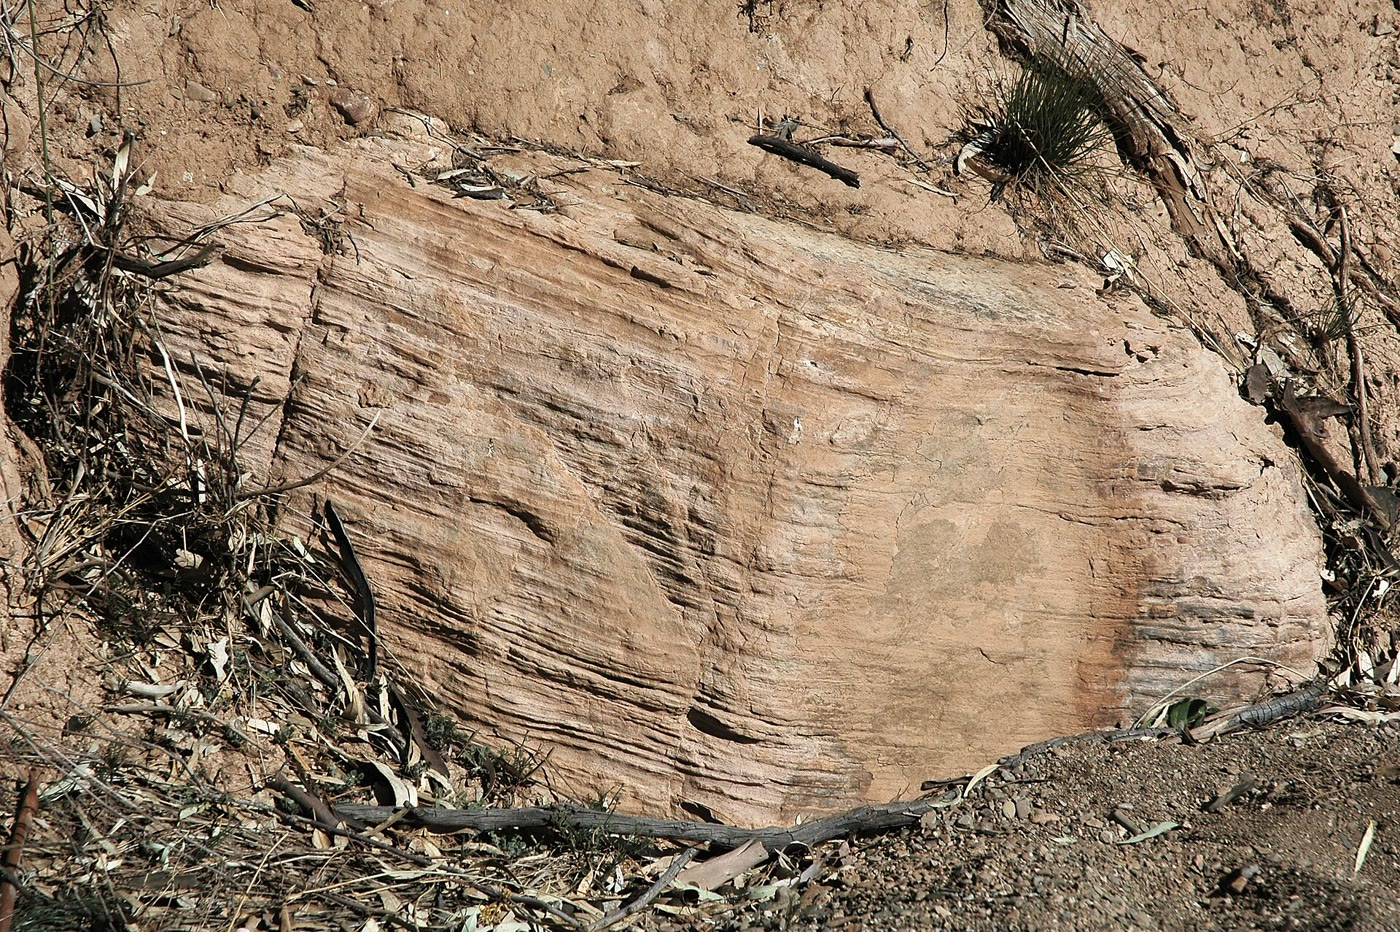
\includegraphics[width=0.66\linewidth]{images/book4/b2-18-cap-carbonate.jpg}
\par\smallskip{\small Un \omterm{def:b2:precambrian-earth:snowball}{carbonato de cobertera}: dolomía laminada de la Formación Nuccaleena,
Flinders Ranges, Australia Meridional, apoyada sobre los depósitos de la glaciación marinoense
(las capas están basculadas). Fotografía de James St.~John, CC~BY~2.0 (Wikimedia Commons).}
\end{omfigure}

Dos bolas de nieve del Criogénico están hoy datadas por edades uranio--plomo en circones de cenizas
volcánicas y por edades renio--osmio en lutitas ricas en materia orgánica. La esturtiense empezó entre 717.5 y
\qty{716.3}{Ma} y terminó entre 659.3 y \qty{658.5}{Ma}: \qty{58}{Myr} de hielo, con el
comienzo y el final sincrónicos en todo el mundo. La marinoense empezó entre 649.9 y
\qty{639.0}{Ma}, con una datación imprecisa, y terminó entre 636.0 y \qty{634.7}{Ma}: al menos
\qty{3}{Myr}. Cada una termina con un único \omterm{def:b2:precambrian-earth:snowball}{carbonato de cobertera}, nunca con varios. Las formaciones de hierro,
ausentes durante mil millones de años, reaparecen en los depósitos glaciares esturtienses. Al menos una bola de nieve
anterior, en el Sidérico, hacia \qty{2.4}{Ga}, coincidió con el GOE; entre ambos
episodios, durante unos \qty{1.5}{Gyr}, casi no se conocen casquetes de hielo.
% ledger: hoffman17:ages, hoffman17:cryochrons, hoffman17:cap, hoffman17:models, hoffman17:earlier

\begin{history}[De una hipótesis extraña a una teoría datada]
En 1964 W.~B. Harland llamó la atención sobre las pruebas de una glaciación del Precámbrico tardío. En
1968 y 1969 M.~I. Budyko, y W.~D. Sellers con un modelo parecido, hallaron que la
\omterm{def:b2:precambrian-earth:ice-albedo}{retroalimentación hielo--albedo} podía hacer que el hielo se extendiera hasta el ecuador una vez que avanzaba lo suficiente; una
Tierra helada globalmente parecía entonces un estado sin retorno, y por tanto uno que nunca había ocurrido.
En 1981 J.~Walker, P.~Hays y J.~Kasting describieron el termostato de la meteorización de los silicatos y
señalaron que en una Tierra helada el dióxido de carbono de los volcanes se acumularía hasta que el hielo
se fundiera: el estado podía terminar por sí mismo. En 1992 J.~L. Kirschvink propuso que había ocurrido
realmente, y lo llamó «Snowball Earth» (\omterm{def:b2:precambrian-earth:snowball}{Tierra bola de nieve}); en 1998 P.~F. Hoffman y sus colegas publicaron
«A Neoproterozoic Snowball Earth», y las épocas panglaciales pasaron a llamarse criocronos. Ningún
depósito glaciar criogénico se había datado radiométricamente antes de 2004; las fechas anteriores son
obra de los años transcurridos desde entonces.
\end{history}
% ledger: hoffman17:history

Los volcanes son la salida. En una Tierra cubierta de hielo, la lluvia y los ríos casi se detienen, y con ellos la
meteorización de los silicatos, y el dióxido de carbono que liberan los volcanes se acumula en el aire
hasta que su efecto invernadero funde el hielo.

\begin{proposition}[Acumulación de dióxido de carbono]\label{prop:b2:precambrian-earth:co2}
Si se libera dióxido de carbono a un ritmo $F$ (masa por año) en una atmósfera de masa
$M_{\text{a}}$ y masa molar media $\bar M$, sin ningún sumidero, el tiempo necesario para llevar su razón de
mezcla en volumen desde casi cero hasta $x$ es
\[
  \tau = \frac{x}{1 - x}\,\frac{M_{\mathrm{CO_2}}}{\bar M}\,\frac{M_{\text{a}}}{F} .
\]
\end{proposition}

\begin{proof}
La atmósfera contiene $n = M_{\text{a}}/\bar M$ moles de otros gases. Añadir $n_c$ moles de
dióxido de carbono hace que su razón de mezcla sea $x = n_c/(n + n_c)$, así que $n_c = n\,x/(1 - x)$, de masa
$n_c M_{\mathrm{CO_2}}$; al ritmo $F$ esto requiere $\tau = n_c M_{\mathrm{CO_2}}/F$.
\end{proof}

\begin{example}[¿Cuánto tarda en escapar?]\label{ex:b2:precambrian-earth:escape}
La estimación preferida más alta de la emisión volcánica actual es de \qty{0.26}{Gt} de dióxido
de carbono al año. Las estimaciones de la
razón de mezcla necesaria para terminar una bola de nieve criogénica van de 0.01 a 0.1. Con $M_{\text{a}} =
\qty{5.1e18}{kg}$, $\bar M = \qty{28.97}{g.mol^{-1}}$ y $M_{\mathrm{CO_2}} =
\qty{44.01}{g.mol^{-1}}$, $x = 0.01$ requiere $\frac{0.01}{0.99}\times1.519\times\qty{5.1e18}{kg}
/ \qty{0.26e12}{kg.yr^{-1}} = \qty{0.30}{Myr}$, y $x = 0.1$ requiere \qty{3.3}{Myr}.
\end{example}
% ledger: usgs:volcanic-co2, hoffman17:co2, earth:Matm, earth:Mmol, ciaaw:abridged-2024
% values: co2_t001_Myr 0.301, co2_t01_Myr 3.311 (precambrian.py)

Una columna de dióxido de carbono puro que pesara \qty{1}{bar} sobre toda la Tierra requeriría
\qty{20}{Myr} al mismo ritmo, la cifra que dieron Walker, Hays y Kasting. Unos pocos millones de años
es mucho tiempo, pero la esturtiense duró \qty{58}{Myr}. O el umbral era más alto, o la
desgasificación menor, o la Tierra helada seguía teniendo sumideros: la meteorización del fondo marino joven,
que no se detiene bajo el hielo, es un candidato. En el modelo de balance energético, la salida requiere
que la emisividad efectiva de la bola de nieve baje hasta que su temperatura alcance \qty{263}{K}: bajo
el Sol criogénico, el \qty{94}{\percent} del actual, de 0.616 a 0.472, un atrapamiento adicional de
unos \qty{39}{W.m^{-2}} (\cref{exo:b2:precambrian-earth:10}).
% ledger: hoffman17:co2, hoffman17:models, usgs:volcanic-co2
% values: one_bar_Myr 19.98, eps_melt_094 0.4716, forcing_melt_094 39.1 (precambrian.py)

Cuando el hielo se abre por fin en el ecuador, la retroalimentación actúa al revés: el mar oscuro absorbe más
luz solar, el hielo retrocede, y en los modelos la línea del hielo corre hacia los polos en unos
\qty{2}{kyr}. La Tierra se encuentra entonces con un enorme efecto invernadero sobre una superficie oscura, unas
secuelas cálidas. La meteorización, muy rápida en ese clima, vierte calcio, magnesio y bicarbonato en
el mar, donde precipitan los \omterm{def:b2:precambrian-earth:snowball}{carbonatos de cobertera} mientras el agua de fusión inunda las plataformas; hacen falta
unos diez millones de años para volver a bajar el dióxido de carbono. Los casquetes de hielo y los \omterm{def:b2:precambrian-earth:snowball}{carbonatos de
cobertera}, las formaciones de hierro y las edades sincrónicas son la razón por la que la mayoría de los geólogos aceptan hoy
que las bolas de nieve criogénicas ocurrieron, aunque todavía se discute lo extremas que fueron ---si sobrevivió un cinturón de aguas
abiertas en el ecuador, como proponen los modelos de «cinturón de agua» (\textit{waterbelt})---.
% ledger: hoffman17:hysteresis, hoffman17:cap, hoffman17:debate

\section*{Ejercicios}\label{sec:b2:precambrian-earth:exercises}

Datos para los ejercicios, salvo indicación contraria: $\sigma = \qty{5.670e-8}{W.m^{-2}.K^{-4}}$;
$S_0 = \qty{1361}{W.m^{-2}}$; albedo actual 0.294 y temperatura media de la superficie \qty{288}{K};
albedo de la bola de nieve 0.6; rampa de \qty{263}{K} a \qty{283}{K}; emisividad efectiva actual
0.616; ley de Gough $L/L_0 = 1/(1 + 0.4\,t/t_\odot)$ para un tiempo $t$ antes del presente, $t_\odot =
\qty{4.567}{Gyr}$; liquidus de las \omterm{def:b2:precambrian-earth:greenstone}{komatiitas} \qty{1616}{\celsius} con \qty{32.2}{\percent} de MgO,
pendiente \qty{18.0}{\celsius} por punto porcentual; periodos de semidesintegración \ce{^{238}U} \qty{4.468}{Gyr}, \ce{^{235}U}
\qty{0.704}{Gyr}, \ce{^{232}Th} \qty{14.0}{Gyr}, \ce{^{40}K} \qty{1.248}{Gyr}.
% ledger: const:sigma, earth:TSI, earth:albedo, earth:Tsurf, hoffman17:models, gough81:luminosity, connelly12:cai, so16:liquidus, iaea:isotopes

\begin{exercise}[$\star$]\label{exo:b2:precambrian-earth:1}
(a) ¿Cuánto duraron el \omterm{def:b2:precambrian-earth:eons}{Hádico}, el \omterm{def:b2:precambrian-earth:eons}{Arcaico} y el \omterm{def:b2:precambrian-earth:eons}{Proterozoico}? (b) ¿Qué fracción de la edad
de la Tierra suman los tres? (c) ¿Qué edad tenía la Tierra cuando cristalizó el circón más antiguo conocido,
y cuando se formaron las rocas más antiguas?
\end{exercise}

\begin{exercise}[$\star$]\label{exo:b2:precambrian-earth:2}
Hoy la \omterm{def:b2:elements-in-the-earth:bse}{Tierra silicatada global} libera, por kilogramo, \qty{1.917}{pW} del \ce{^{238}U},
\qty{0.082}{pW} del \ce{^{235}U}, \qty{2.089}{pW} del \ce{^{232}Th} y \qty{0.818}{pW} del
\ce{^{40}K} ($\qty{1}{pW} = \qty{e-12}{W}$). (a) Hállese cada contribución hace \qty{3}{Gyr}, y
el total. (b) ¿En qué factor ha disminuido desde entonces la producción de calor? (c) ¿Qué isótopo domina
hoy, y cuál dominaba entonces?
\end{exercise}

\begin{exercise}[$\star$]\label{exo:b2:precambrian-earth:3}
Úsese el termómetro de las \omterm{def:b2:precambrian-earth:greenstone}{komatiitas}. (a) ¿Cuál es el liquidus de una \omterm{def:b2:precambrian-earth:greenstone}{komatiita} con un
\qty{28}{\percent} de MgO? (b) ¿Qué contenido en MgO corresponde a \qty{1500}{\celsius}? (c) Una
colada con textura spinifex tiene un MgO de roca total del \qty{38}{\percent}. ¿Por qué no debe leerse
su liquidus en la recta?
\end{exercise}

\begin{exercise}[$\star$]\label{exo:b2:precambrian-earth:4}
Ordénense los acontecimientos siguientes y dense sus edades aproximadas: el \omterm{def:b2:precambrian-earth:goe}{Gran Evento de Oxidación}, los
primeros estromatolitos, el final de la glaciación marinoense, las últimas \omterm{def:b2:precambrian-earth:greenstone}{komatiitas} comunes, las
rocas más antiguas, el segundo aumento del oxígeno, los primeros fósiles ediacáricos, el final de las estructuras de domos y
quillas de Pilbara.
\end{exercise}

\begin{exercise}[$\star\star$]\label{exo:b2:precambrian-earth:5}
(a) Compruébese que la emisividad efectiva de la Tierra actual es 0.616. (b) Hállese el equilibrio de bola de
nieve bajo el Sol actual. (c) Demuéstrese que el equilibrio intermedio, \qty{275.5}{K}, cumple
$R = E$ con un margen de \qty{0.5}{W.m^{-2}}. (d) Hállense allí las pendientes de $R$ y de $E$, y conclúyase
que es inestable.
\end{exercise}

\begin{exercise}[$\star\star$]\label{exo:b2:precambrian-earth:6}
(a) Con la ley de Gough, hállese la luz solar de hace \qty{2.4}{Ga} y de hace \qty{0.65}{Ga} como fracciones
de la actual. (b) En el modelo, ¿es posible un clima cálido en cada fecha con la emisividad actual?
(c) Hoffman y sus colegas escriben que el Sol sidérico era alrededor de un \qty{10}{\percent} más débil que
el Sol criogénico. Compruébese.
\end{exercise}

\begin{exercise}[$\star\star$]\label{exo:b2:precambrian-earth:7}
La esturtiense duró de \qty{716.9}{Ma} a \qty{658.9}{Ma} (puntos medios de los intervalos datados),
y la marinoense de \qty{644.5}{Ma} a \qty{635.4}{Ma}. (a) Hállense sus duraciones y el
interglaciar entre ambas. (b) ¿Durante qué fracción del periodo Criogénico, de 720 a \qty{635}{Ma},
cubrió el hielo la Tierra, según estas cifras? (c) ¿Por qué la duración de la marinoense es solo una
cifra aproximada?
\end{exercise}

\begin{exercise}[$\star\star$]\label{exo:b2:precambrian-earth:8}
(a) ¿Cuánto tardan los volcanes, a \qty{0.26}{Gt} al año y sin sumidero, en llevar el aire a
una razón de mezcla de dióxido de carbono de 0.05? (b) ¿Cuántas veces las \qty{278}{ppm} de 1750 es eso? (c) Si la mitad de la emisión la absorbiera la meteorización del fondo
marino, ¿cuánto tardarían?
\end{exercise}
% ledger: usgs:volcanic-co2, earth:Matm, earth:Mmol, ciaaw:abridged-2024, ipcc:erf-2xco2

\begin{exercise}[$\star\star$]\label{exo:b2:precambrian-earth:9}
Una diamictita neoproterozoica contiene cantos estriados, algunos de los cuales descansan en un barro finamente laminado
que se curva hacia abajo bajo ellos. (a) ¿Qué indica esa curvatura? (b) Su paleolatitud es
\ang{10}. ¿Por qué importa para la hipótesis de la bola de nieve? (c) Está recubierta directamente por una
dolomía laminada rosada de unos pocos metros de espesor. ¿Qué es, y qué registra?
\end{exercise}

\begin{exercise}[$\star\star\star$]\label{exo:b2:precambrian-earth:10}
Bajo el Sol criogénico, $S = 0.94\,S_0$. (a) Demuéstrese que en el modelo el estado cálido todavía
existe, por poco, pero que también existe una bola de nieve. (b) Hállese la temperatura de la bola de nieve con la
emisividad actual. (c) Hállese la emisividad con la que la bola de nieve alcanza \qty{263}{K} y
se deshiela. (d) Conviértase el cambio de emisividad en un atrapamiento adicional de radiación de onda larga a
\qty{263}{K}, en \unit{W.m^{-2}}.
\end{exercise}

\begin{exercise}[$\star\star\star$]\label{exo:b2:precambrian-earth:11}
(a) Con los puntos de inflexión de la \cref{prop:b2:precambrian-earth:tipping}, demuéstrese que la anchura
del bucle de histéresis, $S_{\text{m}}/S_{\text{f}}$, no depende de la emisividad, y
calcúlese. (b) ¿Qué haría más estrecho el bucle? (c) ¿Por qué una bola de nieve solo puede deshelarse lejos de
las condiciones en que se heló?
\end{exercise}

\begin{exercise}[$\star\star\star$]\label{exo:b2:precambrian-earth:12}
Dedúzcase la constante de tiempo del modelo de balance energético cerca del equilibrio cálido, $\tau =
C/(E'(T^*) - R'(T^*))$, y evalúese para una capa de mezcla oceánica de \qty{50}{m} de profundidad, de densidad
\qty{1025}{kg.m^{-3}} y calor específico \qty{3992}{J.kg^{-1}.K^{-1}}. ¿Qué le ocurre a $\tau$ cuando la
luz solar se acerca al punto de inflexión izquierdo, en este modelo y en un modelo cuyo albedo varía
de forma continua con la temperatura?
\end{exercise}
% ledger: noaa:seawater-1025, teos10:cp0

\begin{problem}[{Problema de fin de semana --- Una Tierra joven más caliente}]\label{pb:b2:precambrian-earth:1}
Este problema sigue a la Tierra joven desde su interior hasta su aire. Úsense los datos de los
ejercicios; la \omterm{def:b2:elements-in-the-earth:bse}{Tierra silicatada global} contiene \qty{0.0203}{ppm} de uranio, \qty{0.0795}{ppm} de
torio y \qty{240}{ppm} de potasio en masa, y sus isótopos liberan \qty{95.13}{\micro W}
(\ce{^{238}U}), \qty{568.47}{\micro W} (\ce{^{235}U}), \qty{26.28}{\micro W} (\ce{^{232}Th}) y
\qty{28.47}{\micro W} (\ce{^{40}K}) por kilogramo de isótopo. En masa, el uranio es
\qty{99.29}{\percent} \ce{^{238}U} y \qty{0.711}{\percent} \ce{^{235}U}, y el potasio,
\qty{0.0120}{\percent} \ce{^{40}K}. Redondéese a tres cifras significativas.

\noindent\textbf{Parte I --- El calor del interior.}
\begin{enumerate}
  \item Hállese el calor liberado hoy por cada isótopo por kilogramo de \omterm{def:b2:elements-in-the-earth:bse}{Tierra silicatada global}, en
        \unit{pW.kg^{-1}}.
  \item Hállese el total.
  \item Hállese la constante de desintegración de cada isótopo, en \unit{Gyr^{-1}}.
  \item Hállese cada contribución hace \qty{2.7}{Gyr}, cuando entraron en erupción las \omterm{def:b2:precambrian-earth:greenstone}{komatiitas} de Pyke Hill.
  \item Hállense el total de entonces y su razón con el actual.
  \item ¿Qué isótopo daba más calor entonces? ¿Por qué da tan poco hoy?
\end{enumerate}

\noindent\textbf{Parte II --- El Sol del Arcaico.}
\begin{enumerate}[resume]
  \item Con la ley de Gough, hállese la luz solar de hace \qty{2.7}{Ga} como fracción de la actual, y en
        \unit{W.m^{-2}}.
  \item Hállese el equilibrio cálido con esa luz solar y la emisividad actual. ¿Es un estado cálido
        válido del modelo?
  \item Hállese el equilibrio de bola de nieve con esa luz solar.
  \item ¿Qué emisividad efectiva mantendría la Tierra a \qty{288}{K} con el albedo cálido?
  \item El dióxido de carbono por sí solo podría haberlo logrado con 0.004 a \qty{0.03}{bar} a \qty{2.5}{Ga}.
        En una atmósfera de alrededor de \qty{1}{bar}, ¿cuántas veces las \qty{278}{ppm} de 1750 es
        eso?
  \item Nómbrese el proceso que mantuvo el dióxido de carbono en ese nivel durante cientos de millones
        de años.
\end{enumerate}

\noindent\textbf{Parte III --- Una bola de nieve y su final.}
\begin{enumerate}[resume]
  \item La primera bola de nieve, hace \qty{2.4}{Ga}: hállese la luz solar de entonces como fracción de la actual.
        ¿Sigue siendo posible el estado cálido del modelo con la emisividad actual?
  \item A \qty{0.26}{Gt} de dióxido de carbono al año, ¿cuánto se tarda en alcanzar una razón de
        mezcla de 0.1?
  \item Si el umbral bajo el Sol sidérico, más débil, era el doble, 0.2, ¿cuánto se tarda?
  \item ¿Qué roca registra el final de una bola de nieve, y cómo?
  \item ¿Por qué las formaciones de hierro esturtienses necesitan un océano sin oxígeno bajo el hielo?
\end{enumerate}

\noindent\textbf{Parte IV --- El termómetro de las komatiitas.}
\begin{enumerate}[resume]
  \item Compruébese la pendiente de la recta de las \omterm{def:b2:precambrian-earth:greenstone}{komatiitas} a partir de los dos experimentos.
  \item Un líquido komatiítico de Pyke Hill tenía un \qty{30}{\percent} de MgO. Hállese su liquidus.
  \item Hállese el liquidus de la \omterm{def:b2:precambrian-earth:greenstone}{komatiita} de Barberton, con un \qty{32.2}{\percent} de MgO.
  \item Hállese el liquidus de un basalto primario de dorsal con un \qty{12}{\percent} de MgO.
  \item Con la pendiente del Kilauea, \qty{20}{\celsius} por punto porcentual, ¿qué temperatura tendría el
        basalto, partiendo del punto de Barberton? ¿Cuánto importa la elección de la pendiente?
  \item ¿Por qué la diferencia de temperatura entre las dos lavas es mayor que la diferencia de
        temperatura potencial entre el manto arcaico y el actual?
  \item En resumen: ¿cuánto más caliente era la lava komatiítica arcaica más caliente que un basalto primario
        de las dorsales actuales?
\end{enumerate}
\end{problem}
% ledger: ms95:pm-trace, dye:isotope-heat, iaea:isotopes, gough81:luminosity, cz20:archean-air, ipcc:erf-2xco2, usgs:volcanic-co2, hoffman17:co2, so16:liquidus, helz98:glass-thermometer, pierru22:komatiite
